\begingroup
\let\clearpage\relax
\chapter{Projekt komputera 8-bitowego - zarys problematyki}
\section{Historia rozwoju komputerów osobistych}

W latach 80' ubiegłego wieku, nastąpił znaczny wzrost ilości osób posiadających komputer osobisty. 'Apple I', jeden z pierwszych komputerów osobistych, stworzony przez Steve'a Wozniaka w 1976 roku, był przeznaczony głównie dla tak zwanych hobbystów, ze względu na potrzebę samodzielnego montażu jego komponentów. Jego rewolucyjność polegała na nowatorskim podejściu do kontaktu z użytkownikiem, jako jeden z pierwszych komputerów wykorzystywał klawiaturę oraz monitor jako urządzenia peryferyjne, co pozwoliło na znacznie wygodniejszą obsługę.  Jego sukces zapoczątkował rozwój komputerów osobistych, które zaczęły pojawiać się na rynku w coraz większej liczbie.
\begin{figure}[h]
    \centering
    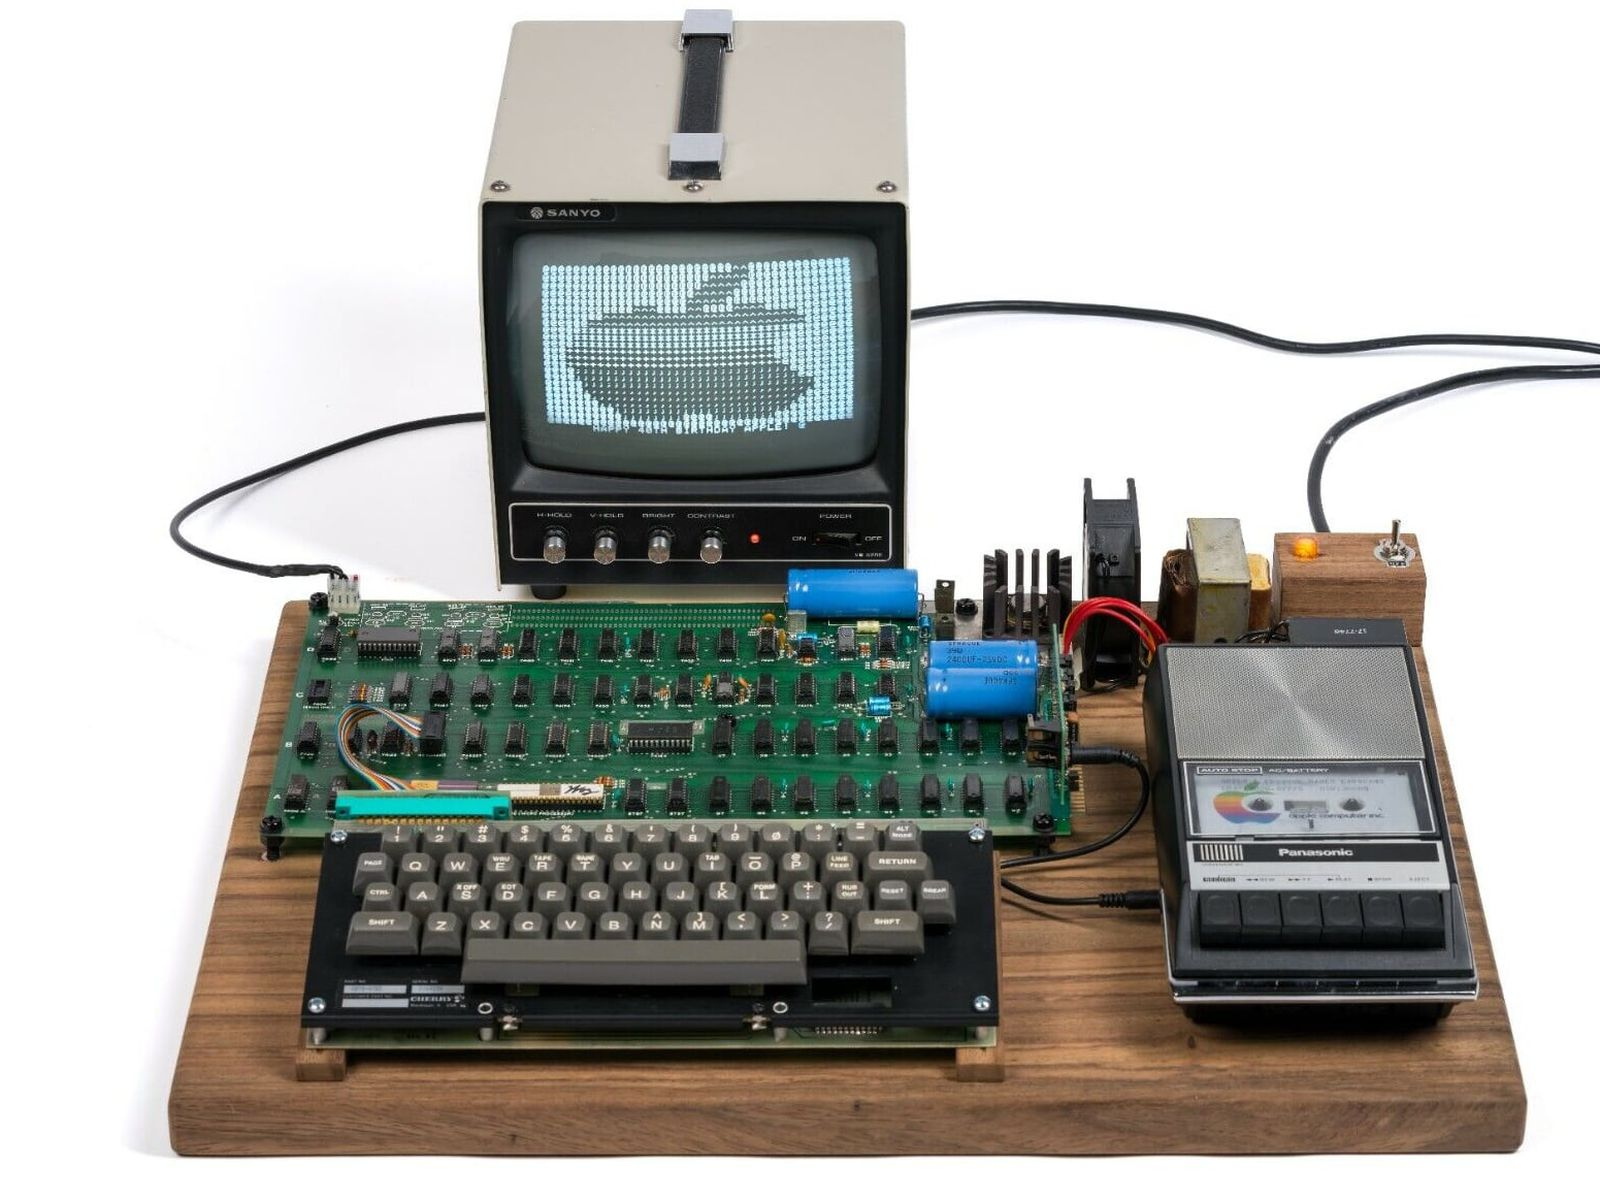
\includegraphics[width=0.8\textwidth]{images/apple-1.jpg} % Wstaw nazwę pliku z obrazem
    \caption{ \textit{Apple-1}}
    \label{fig:apple1} 
    \vspace{0.5em} % Odstęp między podpisem a źródłem
    \footnotesize Źródło: \parencite{macrumors2016}
\end{figure}
Czy 'Apple II', który umożliwia wyświetlanie kolorowego obrazu na monitorze, umożliwi odtwarzanie dźwięku, czy nawet pozwoli na użycie kart rozszerzeń. Na rynku pojawił się także komputer 'BBC Micro', stworzony we współpracy z brytyjską stacją BBC, którego głównym celem była edukacja i nauka programowania. Dzięki powyższym modelom komputerów osobistych stawały się one coraz bardziej przystępne cenowo i dostępne dla szerokiego grona użytkowników.
Wszystkie te komputery łączyła jedna cecha wspólna – procesor MOS 6502, który znacznie obniżał koszty produkcji. Dzięki temu urządzenia takie jak „Apple I”, „Commodore 64”, „BBC Micro” itp. były dostępne w znacznie niższych cenach, co czyniło je popularnymi nie tylko wśród entuzjastów technologii, ale także w codziennym użytkowaniu. Dostępność ta przyczyniła się do szybkiego wzrostu liczby użytkowników komputerów i stanowiła ważny krok w rozwoju technologii komputerowej.

\null\newpage
\section{Wybór procesora MOS 6502 jako kluczowego elementu projektu.}

Początki komputerów osobistych zdominowały głównie dwa procesory, MOS 6502 oraz procesor Zilog Z80. Procesor firmy MOS, teraz wykupionej przez firmę Western Design Center, jest dalej produkowany oraz dostępny w sprzedaży. Firma Zilog wycofała się z produkcji procesora Z80 na początku 2024 roku \parencite{ithardware2024}. 

\begin{figure}[h]
    \centering
    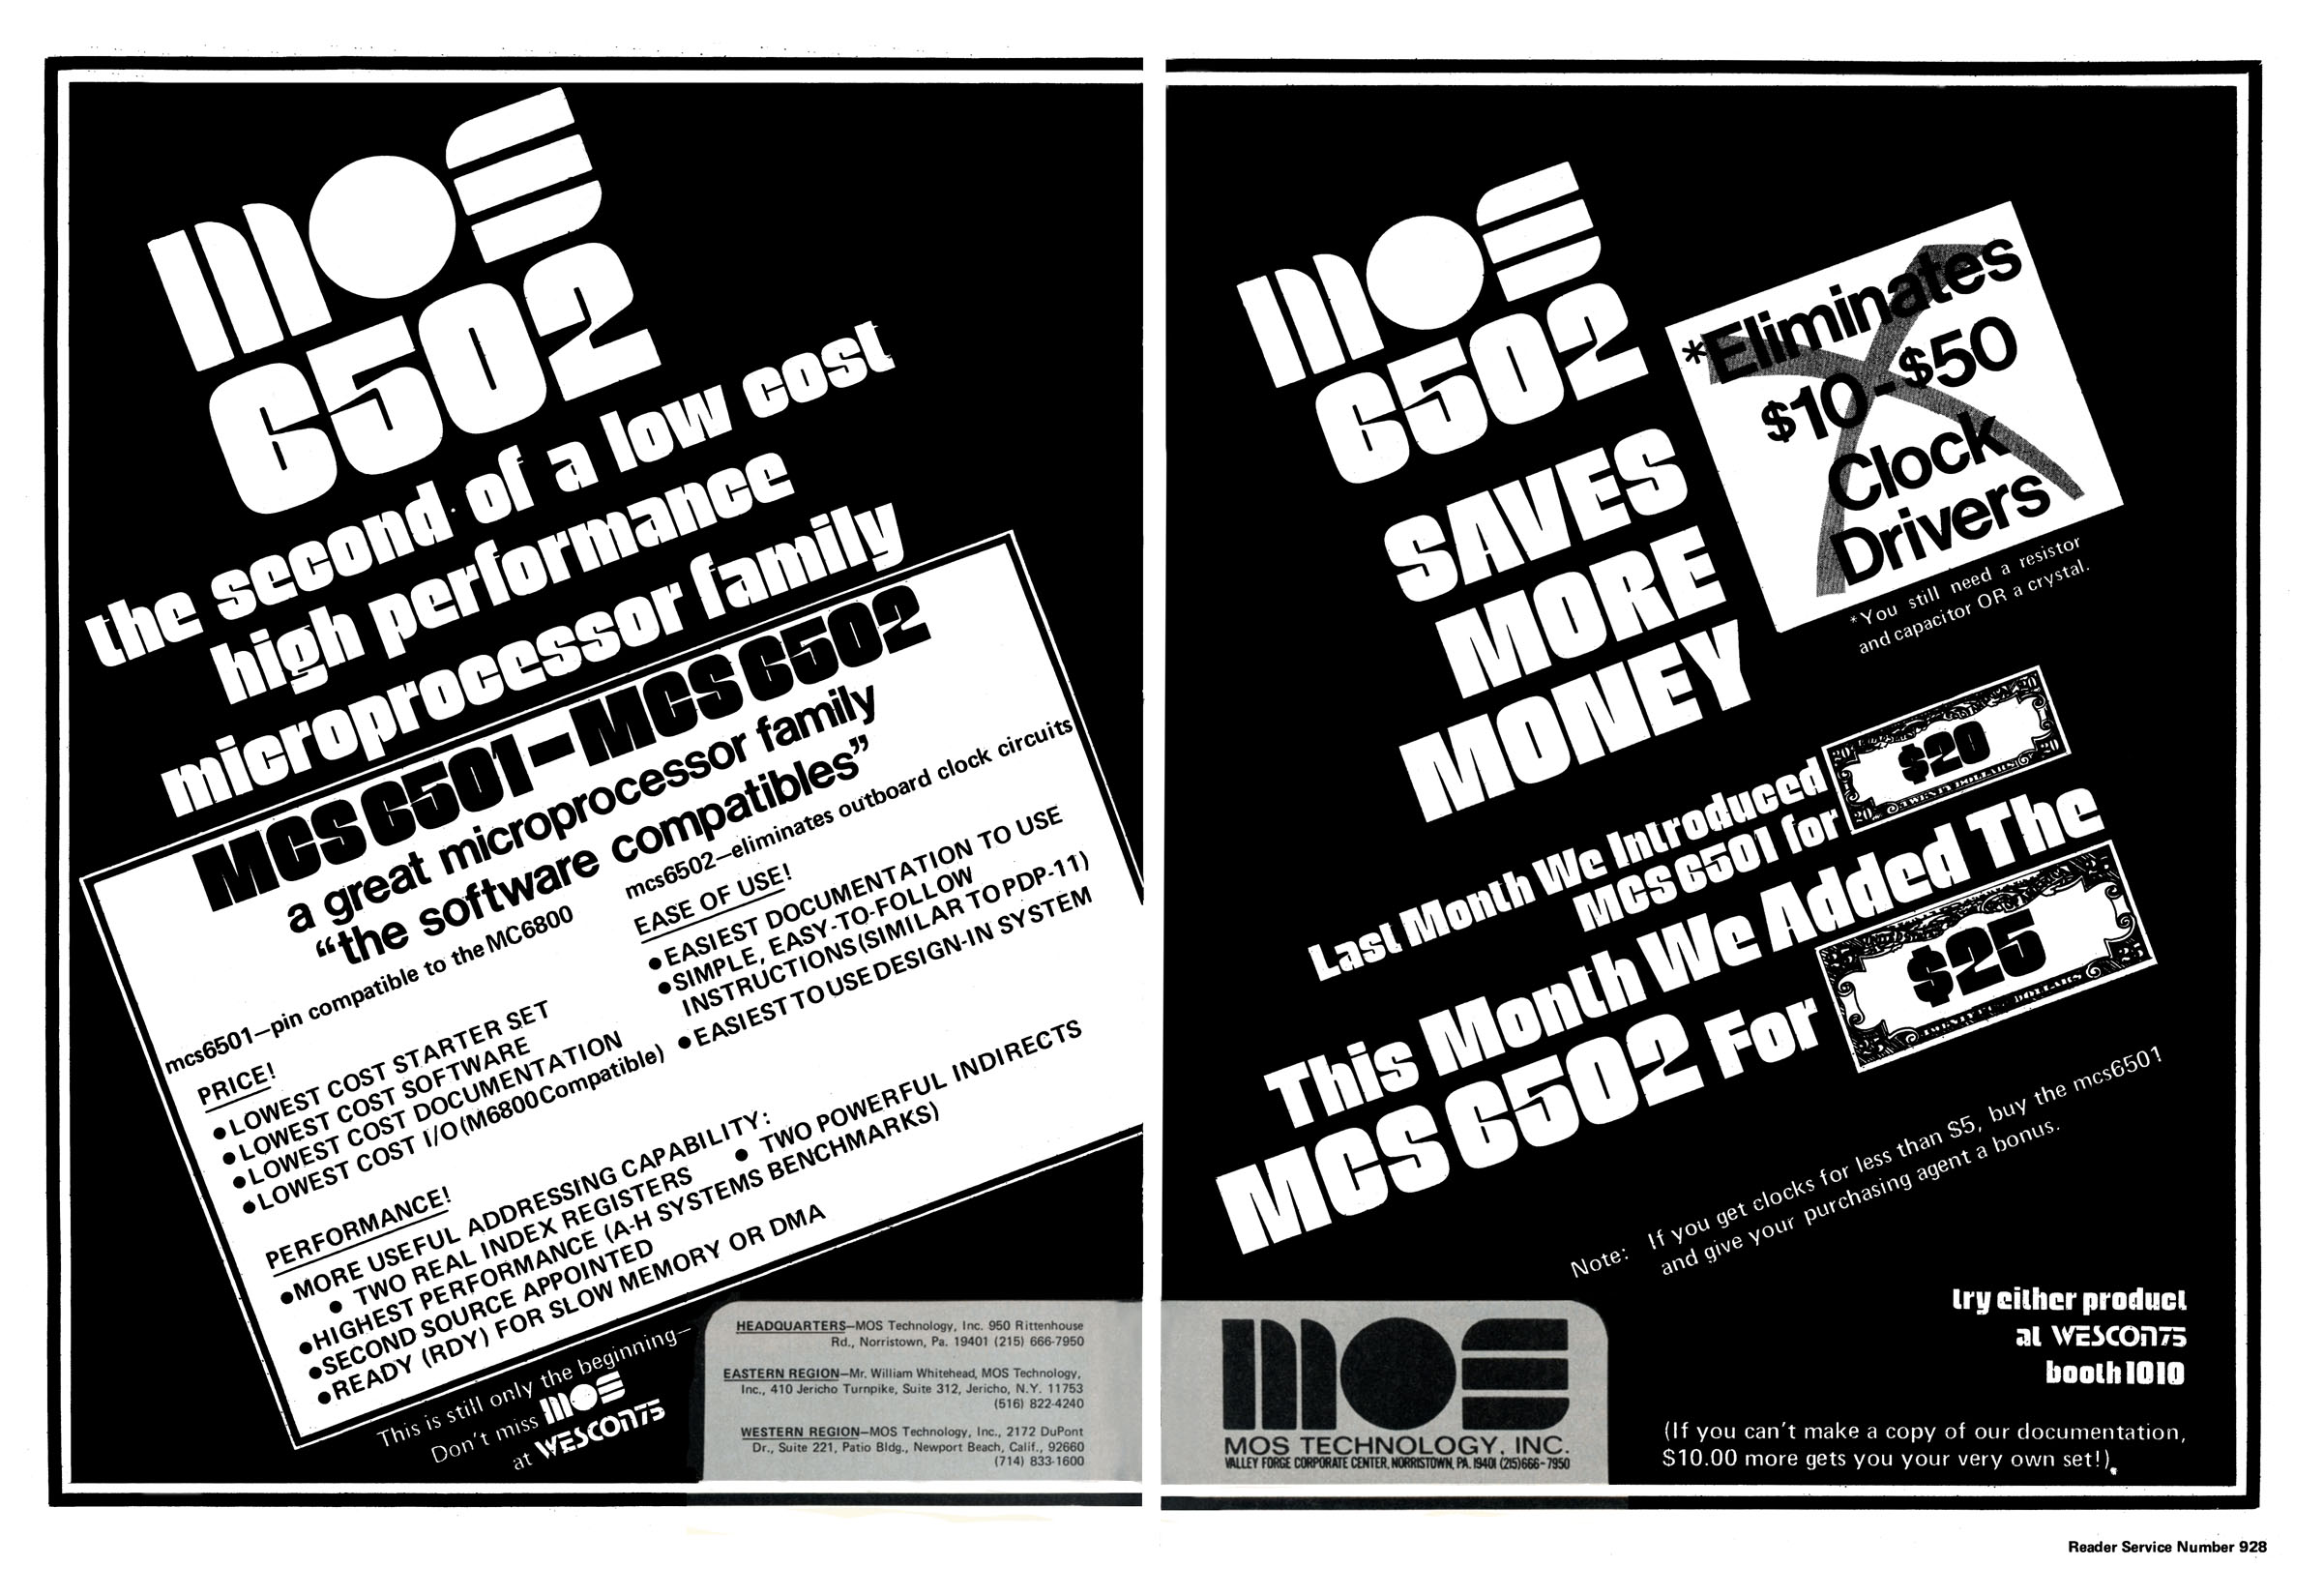
\includegraphics[width=0.8\textwidth]{images/MOS_6501_6502_Ad_Sept_1975.jpg} % Wstaw nazwę pliku z obrazem
    \caption{ \textit{Reklama procesora mos 6502 z 1975 roku}}
    \label{fig:apple1} 
    \vspace{0.5em} % Odstęp między podpisem a źródłem
    \footnotesize Źródło: \parencite{wikipedia6502}
\end{figure}

Procesor 8-bitowy posiada o wiele łatwiejszą architekturę do zrozumienia niż procesor 16-bitowy lub procesor o jeszcze większej magistrali. Rozwiązanie takie umożliwi łatwiejszą pracę nad komputerem. Dzisiaj dalej popularne są mikroprocesory wykorzystujące 8-bitową magistralę, takie jak poprzednio pisane Z80 oraz 65C02 (wersja CMOS układu 6502) oraz chociażby popularny układ ATmega328P w architekturze ARM wykorzystywany w Arduino. Procesor ARM został zaprojektowany przez Sophie Wilson, która także pomagała w tworzeniu BBC Micro. Procesory architektury ARM mają podobny rejestr stanu do procesora 6502. Jednak jest to nie jedyny dowód na podobieństwa tych dwóch procesorów. Inżynierowie firmy Acorn, podczas tworzenia zbioru instrukcji dla procesora ARM\parencite{statusregisterARm}, inspirowali się krótkimi i prostymi instrukcjami w procesorze 6502, które były zbliżone do procesorów architektury RISC \parencite{atack1993}.

\null\newpage
\section{Cele projektu}
Celem niniejszej pracy inżynierskiej jest stworzenie komputera, który umożliwi naukę programowania niskopoziomowego oraz pracy z mikrokontrolerami z rodziny AtMega.

\endgroup